
\documentclass[final]{beamer}

\usepackage[scale=1.24]{beamerposter} % Use the beamerposter package for laying out the poster

%\usetheme{confposter} % Use the confposter theme supplied with this template
%\usetheme[faculty=chemo]{fibeamer} % Uncomment to use Masaryk University's fibeamer theme instead.

%\setbeamercolor{block title}{fg=ngreen,bg=white} % Colors of the block titles
%\setbeamercolor{block body}{fg=black,bg=white} % Colors of the body of blocks
%\setbeamercolor{block alerted title}{fg=white,bg=dblue!70} % Colors of the highlighted block titles
%\setbeamercolor{block alerted body}{fg=black,bg=dblue!10} % Colors of the body of highlighted blocks
% Many more colors are available for use in beamerthemeconfposter.sty

%-----------------------------------------------------------
% Define the column widths and overall poster size
% To set effective sepwid, onecolwid and twocolwid values, first choose how many columns you want and how much separation you want between columns
% In this template, the separation width chosen is 0.024 of the paper width and a 4-column layout
% onecolwid should therefore be (1-(# of columns+1)*sepwid)/# of columns e.g. (1-(4+1)*0.024)/4 = 0.22
% Set twocolwid to be (2*onecolwid)+sepwid = 0.464
% Set threecolwid to be (3*onecolwid)+2*sepwid = 0.708

\newlength{\sepwid}
\newlength{\onecolwid}
\newlength{\twocolwid}
\newlength{\threecolwid}
\setlength{\paperwidth}{46.8in} % A0 width: 46.8in
\setlength{\paperheight}{33.1in} % A0 height: 33.1in
\setlength{\sepwid}{0.024\paperwidth} % Separation width (white space) between columns
\setlength{\onecolwid}{0.21\paperwidth} % Width of one column
\setlength{\twocolwid}{0.451\paperwidth} % Width of two columns
\setlength{\threecolwid}{0.678\paperwidth} % Width of three columns
%\setlength{\topmargin}{-0.5in} % Reduce the top margin size
%-----------------------------------------------------------

\usepackage{graphicx}  % Required for including images

\usepackage{booktabs} % Top and bottom rules for tables

%----------------------------------------------------------------------------------------
%	TITLE SECTION 
%----------------------------------------------------------------------------------------

\usepackage{graphicx}  % Required for including images

\usepackage{booktabs} % Top and bottom rules for tables

\usepackage{here}

\usepackage[utf8]{inputenc}

\usepackage[ngerman]{babel}

\usepackage{xcolor}


\definecolor{ui-blue}{HTML}{1857c4}
\definecolor{ui-red}{HTML}{cc0012}
\setbeamercolor{block title}{fg=white,bg=ui-blue}
\setbeamercolor{block body}{fg=black,bg=}
\definecolor{docker-green}{HTML}{37974c}
\definecolor{docker-red}{HTML}{cd5458}
\definecolor{docker-lb}{HTML}{4c87e1}
\definecolor{docker-db}{HTML}{1111dc}
\definecolor{docker-pu}{HTML}{8c0285}


\title{Docker \& Microservices Cheatsheet} % Poster title

\author{Sebastian Aurin, Marcel Otega Oßwald} % Author(s)

\institute{Hochschule Mannheim, Fakultät für Informatik} % Institution(s)

%----------------------------------------------------------------------------------------

\begin{document}
\addtobeamertemplate{block end}{}{\vspace*{2ex}} % White space under blocks
\addtobeamertemplate{block example end}{}{\vspace*{2ex}} % White space under example blocks
\addtobeamertemplate{block alerted end}{}{\vspace*{2ex}} % White space under highlighted (alert) blocks

\setlength{\belowcaptionskip}{2ex} % White space under figures
\setlength\belowdisplayshortskip{2ex} % White space under equations
%\begin{darkframes} % Uncomment for dark theme, don't forget to \end{darkframes}
\begin{frame} % The whole poster is enclosed in one beamer frame

%==========================Begin Head===============================
  \begin{columns}
   \begin{column}{\linewidth}
    \vskip1cm
    \centering
    \usebeamercolor{title in headline}{\color{fg}\Huge{\textbf{\inserttitle}}\\[0.5ex]}
    \usebeamercolor{author in headline}{\color{fg}\Large{\insertauthor}\\[1ex]}
    \usebeamercolor{institute in headline}{\color{fg}\large{\insertinstitute}\\[1ex]}
    \vskip1cm
   \end{column}
   \vspace{1cm}
  \end{columns}
 \vspace{1cm}

%==========================End Head===============================

\begin{columns}[t] % The whole poster consists of three major columns, the second of which is split into two columns twice - the [t] option aligns each column's content to the top

\begin{column}{\sepwid}\end{column} % Empty spacer column

\begin{column}{\onecolwid} % The first column

%----------------------------------------------------------------------------------------
%	OBJECTIVES
%----------------------------------------------------------------------------------------

\begin{block}{Microservices ohne Docker}

\begin{itemize}
	\item Deployment und Services beeinflussen sich gegenseitig im Laufzeitverhalten
	\item Ein Service kann alle Services zum Ausfall bringen
	\item Einzelne Services können nicht skaliert werden
	\item Mögliche Konflikte in den Abhängigkeiten
\end{itemize}

\begin{figure}
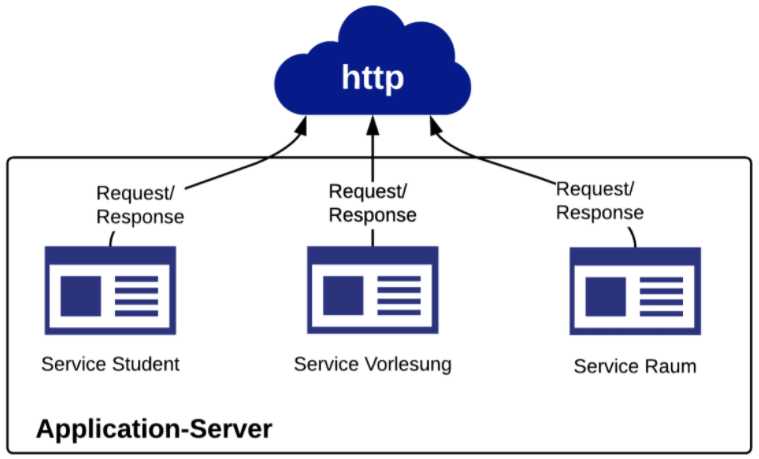
\includegraphics[scale=0.75]{as}	
\end{figure}

\begin{itemize}
\item Hoher Aufwand für System-Konfiguration, Deployment und Monitoring
\item Sehr ressourcenhungrig, jeder Service eigene Ablaufumgebung und Abhängigkeiten
\item Beeinflussen sich gegenseitig im Laufzeitverhalten
\end{itemize}

\begin{figure}
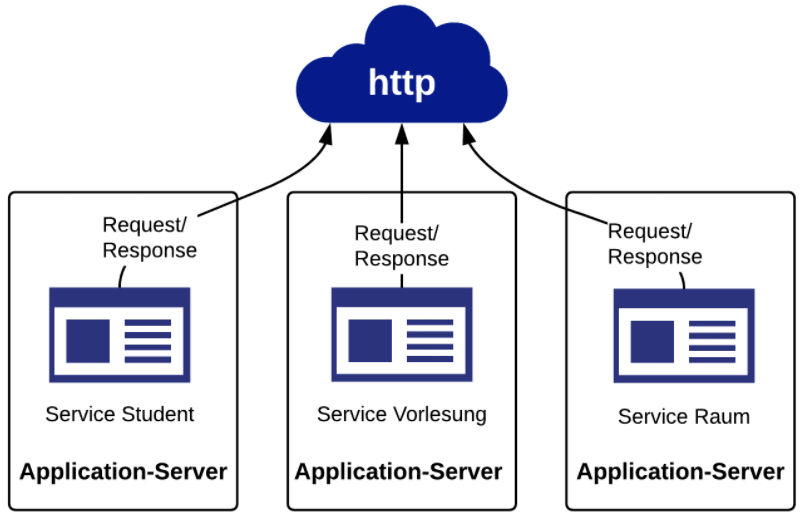
\includegraphics[scale=0.75]{as_mu}	
\end{figure}

\begin{itemize}
\item Sehr ressourcenhungrig, jede VM benötigt eigenes Betriebssystem
\end{itemize}

\begin{figure}
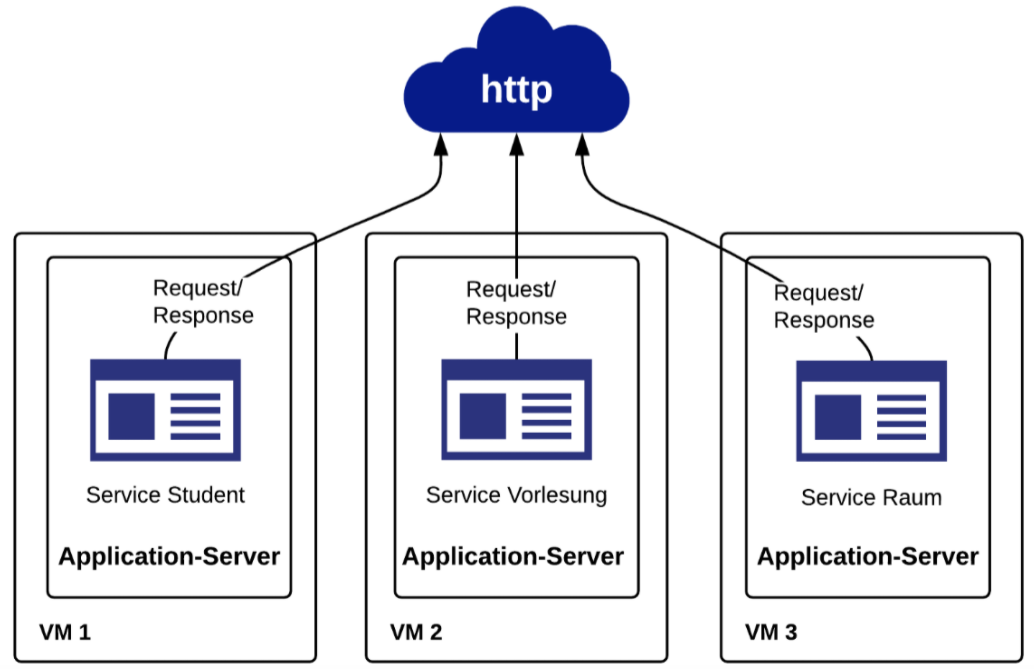
\includegraphics[scale=0.60]{as_vm}	
\end{figure}



\end{block}


\end{column} % End of the first column

\begin{column}{\sepwid}\end{column} % Empty spacer column

\begin{column}{\twocolwid} % Begin a column which is two columns wide (column 2)

\begin{columns}[t,totalwidth=\twocolwid] % Split up the two columns wide column

\begin{column}{\onecolwid}\vspace{-.74in} % The first column within column 2 (column 2.1)

%----------------------------------------------------------------------------------------
%	MATERIALS
%----------------------------------------------------------------------------------------



\begin{block}{Docker Compose}

Mit einer docker-compose-Datei können mehrere Container automatisiert gestartet werden. Diese können dabei auch automatisch verlinkt werden, es können Volumes gemountet oder Ports freigegeben werden und vieles mehr. Auf diese Weise, kann man mit einem einzigen Befehl, \textbf{docker-compose up -d}, alle seine Container starten.
\vspace{2cm}
\par version: \textcolor{docker-db}{'3'} \\
\textcolor{docker-pu}{services:} \\
\hspace{1cm} beispiel-container \\
\hspace{2cm} \textcolor{docker-pu}{image:}java\textcolor{docker-pu}{:}\textcolor{docker-green}{8} \\
\hspace{2cm} \textcolor{docker-pu}{ports:} \\
\hspace{3cm} - \textcolor{docker-green}{8080}\textcolor{docker-pu}{:}\textcolor{docker-green}{8080} \\
\hspace{2cm} \textcolor{docker-pu}{volumes:} \\
\hspace{3cm} - /var/lib/docker/data\textcolor{docker-pu}{:}/var/lib/appdata \\
\hspace{2cm} \textcolor{docker-pu}{links:} \\
\hspace{3cm} - mysql-container \\
\hspace{2cm} \textcolor{docker-pu}{deploy:} \\
\hspace{3cm} \textcolor{docker-pu}{replicas: }\textcolor{docker-green}{5} \\
\hspace{3cm} \textcolor{docker-pu}{restart\_policy:} \\
\hspace{4cm} \textcolor{docker-pu}{condition:} on-failure\\
\hspace{2cm} \textcolor{docker-pu}{command:} [\textcolor{docker-db}{'java'}, \textcolor{docker-db}{'-jar'}, \textcolor{docker-db}{'app.jar'}]\\
\vspace{1.5cm}
\begin{itemize}
	\item \textbf{image} gibt das Baseimage an, das für den Container verwendet werden
	\item \textbf{ports} mappt einen Port vom Host auf den Container
	\item \textbf{volumes} mountet ein Volume, um Daten zu persistieren
	\item \textbf{links} verlinkt den angegebenen Container mit dem aktuellen Container
	\item \textbf{replicas} gibt an wieviele Kopien gestartet werden sollen, wenn es als Stack auf einem Manager gestartet wird
	\item \textbf{restart\_policy} gibt an, ob bzw. wann der Container neu gestartet werden soll
command definiert den Startbefehl

\end{itemize}

\end{block}
%----------------------------------------------------------------------------------------

\end{column} % End of column 2.1
\begin{column}{\sepwid}\end{column} % Empty spacer column

\begin{column}{\onecolwid}\vspace{-.74in} % The second column within column 2 (column 2.2)

%----------------------------------------------------------------------------------------
%	METHODS
%----------------------------------------------------------------------------------------
\begin{block}{Docker Swarm - Grundkonzept}

\par Als erste Ausgangslage hat man ein oder mehrere Dockerfiles erstellt. Da jedes Dockerfile einzeln gebaut und gestartet werden muss, ist der nächste Schritt eine docker-compose.yml - Datei zu erstellen, die mithilfe der Dockerfiles alle Images automatisch erzeugt und die Container startet, inkl. Verlinken, Portmapping und allem was sonst beim Starten von Containern zu beachten ist. Außerdem werden an dieser Stelle auch deploy-Befehle in der Compose-Datei berücksichtigt. Mithilfe von docker stack kann im nächsten Schritt die Compose-Datei auf einem Swarm Manager ausgerollt werden. Ab diesem Punkt kann man den Swarm um beliebige Worker erweitern, auf denen dann auch die Container ausgeführt werden.

\begin{figure}
	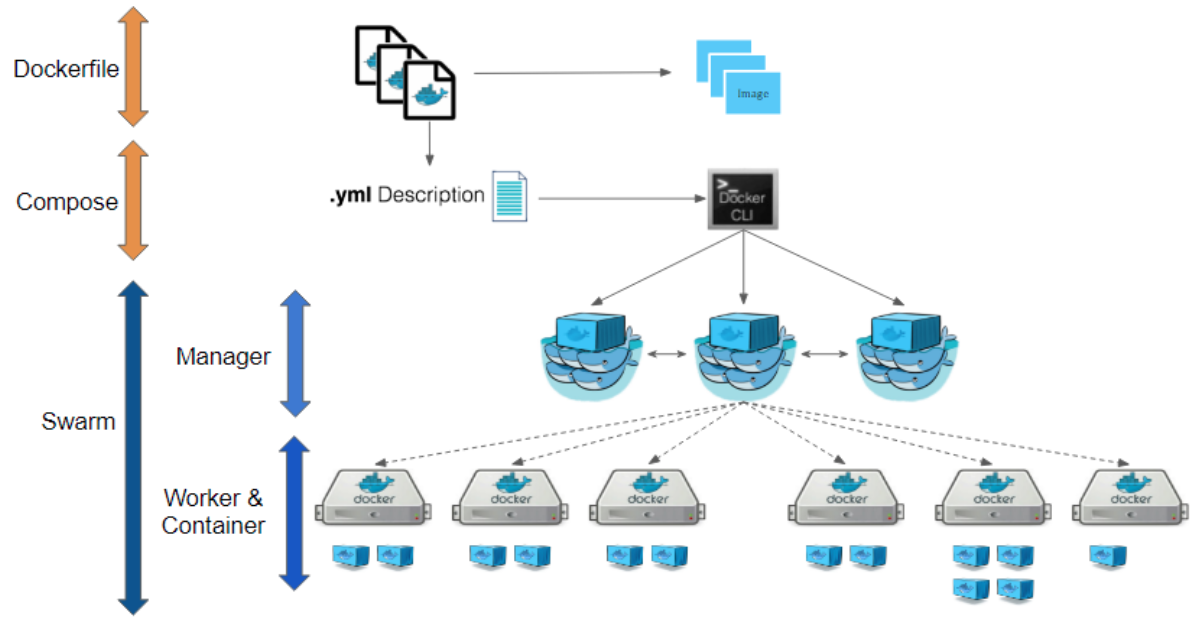
\includegraphics[scale=0.60]{gs}
\end{figure}


\end{block}

\begin{block}{Docker Stack- \& Swarm-Befehle}
\small
\begin{itemize}
	\item \textbf{\$ docker stack deploy -c docker-compose.yml stackname1} -- startet die angegebene Compose-Datei auf einem (Swarm) Manager
	\item \textbf{\$ docker stack ls} -- zeigt alle Stacks an
	\item \textbf{\$ docker stack ps stackname1} -- zeigt alle Container auf dem Stack an
	\item \textbf{\$ docker stack rm stackname1} -- löscht einen Stack und alle seine Container\end{itemize}
\begin{itemize}
\item \textbf{\$ docker swarm init} -- initialisiert einen swarm
\item \textbf{\$ docker swarm leave} -- force entfernt einen Swarm
\end{itemize}


\end{block}


%----------------------------------------------------------------------------------------

\end{column} % End of column 2.2

\end{columns} % End of the split of column 2 - any content after this will now take up 2 columns width

%----------------------------------------------------------------------------------------
%	IMPORTANT RESULT
%----------------------------------------------------------------------------------------



%----------------------------------------------------------------------------------------

\begin{columns}[t,totalwidth=\twocolwid] % Split up the two columns wide column again

\begin{column}{\onecolwid} % The first column within column 2 (column 2.1)

%----------------------------------------------------------------------------------------
%	MATHEMATICAL SECTION
%----------------------------------------------------------------------------------------


%----------------------------------------------------------------------------------------

\end{column} % End of column 2.1
\begin{column}{\sepwid}\end{column} % Empty spacer column

\begin{column}{\onecolwid} % The second column within column 2 (column 2.2)


\end{column} % End of column 2.2

\end{columns} % End of the split of column 2

\end{column} % End of the second column

\begin{column}{\sepwid}\end{column} % Empty spacer column

\begin{column}{\onecolwid} % The third column

%----------------------------------------------------------------------------------------
%	CONCLUSION
%----------------------------------------------------------------------------------------

\begin{block}{Vorteile die Docker \& Swarm mitbringt}

\begin{itemize}

\item einheitliche Ablaufumgebung
\begin{itemize}
\item weniger Dokumentation notwendig
\item 'Works for me' Syndrom fällt weg
\begin{itemize}
\item Konfigurations- und Kompatibilitätsprobleme sind auf ein Minimum reduziert
\end{itemize}
\end{itemize}
\item Docker kann dutzende Services auf einen Dev-System starten
\begin{itemize}
\item produktive Cluster-Umgebung mit Containern am lokalen Entwicklerrechner nachstellen
\end{itemize}
\item einfache Wartung
\begin{itemize}
\item Entwickler liefern lauffähiges Image
\item Container können einfach zur Laufzeit ausgetauscht werden
\end{itemize}
\item Einheitliche Entwicklungsumgebung mit Docker möglich
\begin{itemize}
\item weniger Aufwand für die Einrichtung der Entwicklungsumgebung
\item spezifische Images für jedes Team möglich
\end{itemize}
\item Testen der Anwendung
\begin{itemize}
\item virtuelle Testserver in denen die Anwendungen automatisiert in Sekunden gestartet werden
\item Bei Bedarf kann für jeden Test ein eigener Container gestartet werden, somit ist es möglich das die Tests sich nicht gegenseitig beeinflussen (isoliert testen)
\end{itemize}
\end{itemize}

\begin{itemize}
	\item blitzschnell Services starten
	\begin{itemize}
\item zusätzliche Instanzen
\item neue Services
\end{itemize}
\item Änderungen der Systemlast
\begin{itemize}
\item kann umgehend darauf reagiert werden
\item Container können bedarfsgerecht  zu- oder abgeschaltet werden (Auto-Scaling)
\end{itemize}
\item bei Softwareprobleme im laufenden Betrieb
\begin{itemize}
\item einfach neuen Service starten
\item nicht langwierig versuchen die Instanz zu reparieren
\item Fehlerlogs können in Ruhe geprüft werden
\end{itemize}
\item einfache zentrale Überwachung der Container ist direkt mit docker stats möglich
\begin{itemize}
\item CPU-Auslastung
\item Speichernutzung/verfügbarer Speicher
\item Netzwerkdatenverkehr
\end{itemize}
\end{itemize}


\begin{figure}
\begin{minipage}[t]{0.40\textwidth}\vspace{0pt} 

\includegraphics[width=0.85\textwidth]{sebastian} 
\begin{center}
	Sebastian Aurin
\end{center}
\end{minipage}\hfill%
\begin{minipage}[t]{0.40\textwidth}\vspace{0pt} 

\includegraphics[width=0.85\textwidth]{marcel} 
\begin{center}
	Marcel Ortega Oßwald
\end{center}
\end{minipage}\hfill%

\end{figure}


\end{block}

%----------------------------------------------------------------------------------------

\end{column} % End of the third column

\begin{column}{\sepwid}\end{column} % Empty spacer column

\end{columns} % End of all the columns in the poster

\end{frame} % End of the enclosing frame
%\end{darkframes} % Uncomment for dark theme
\end{document}
